\section{LoRaMAC}\label{sec:archi-loramac:proto}
\renewcommand{\rightmark}{LoRaMac}

    Cette section décris le protocole MAC mis en place pour les communications LoRa. Ce protocole est donc utilisé pour les communications entre la racine LoRa et les racines RPL. Ces dernières étant contraintes en énergie, leur radio LoRa n'est pas tout le temps allumée. Le protocole prend donc en compte cette contrainte.

\subsection*{Etats d'une Racine RPL}
    Les racines RPL utilisent 4 états illustrés dans le diagramme d'état de la figure~\ref{fig:archi-state}. A l'initiation du réseau, une racine RPL se trouve dans l'état \textit{alone}. Elle demande ensuite son préfixe à la racine LoRa. Si la transmission échoue trop de fois, elle entre dans l'état \textit{sleep} dans lequel ses radios sont éteintes, jusqu'à ce que l'évènement \textit{wake up} soit déclenché pour retourner dans l'état \textit{alone}. Si la transmission est réussie, et donc que le préfixe est reçu, la racine RPL se trouve dans l'état \textit{ready}. Quand une racine RPL envoie une trame qui nécessite un acquittement, tant que celui-ci n'est pas reçu elle se trouvera dans l'état \textit{wait\_response}. Une fois l'acquittement reçu, elle retournera dans l'état \textit{ready}.
    
    Les trames qui doivent être envoyées le seront en fonction de l'état dans lequel se trouve une racine RPL. Dans l'état \textit{ready}, les trames de données peuvent être envoyées, mais ce n'est pas le cas dans les états \textit{alone} et \textit{wait\_response}. En effet dans le premier la racine RPL ne peut pas envoyer de données car elle n'a pas encore rejoint le réseau et dans le second, elle attend une réponse.
    \begin{figure}[H]
        \centering
        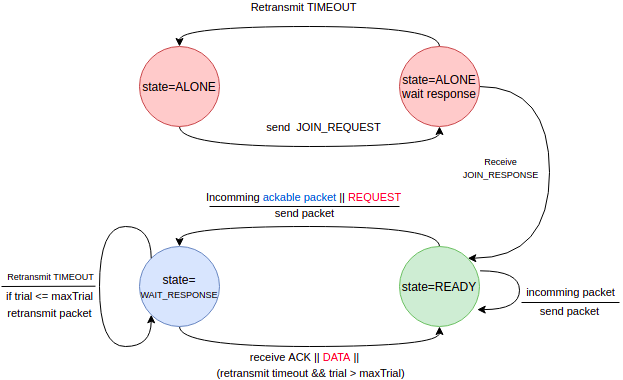
\includegraphics[scale=0.5]{res/pictures/loramac-state.drawio.png}
        \caption{Diagramme d'état des racines RPL.}
        \label{fig:archi-state}
    \end{figure}

\subsection*{Etats de la racine LoRa}
    Le diagramme d'état de la racine LoRa pour chaque racine RPL qui a rejoint le réseau est 
    illustré à la figure~\ref{fig:archi-state-lora}. Une fois que la racine RPL (enfant de la 
    racine LoRa) a rejoint le réseau, l'état est READY. Cela signifie que la racine LoRa est prête 
    à recevoir des données de cet enfant. Si elle reçoit une trame DATA, les données sont 
    transmises à la couche supérieure. Elle peut donc rester dans le même état. Elle reste aussi 
    dans l'état READY si elle reçoit une QUERY et qu'il n'y a aucune données disponible pour cet 
    enfant. En revanche, si des données sont disponibles, la racine LoRa entre dans l'état TRANSMIT 
    dans lequel elle va envoyer tous les paquets disponibles pour cet enfant. Une fois dans l'état 
    TRANSMIT la racine LoRa envoie un paquet et bascule dans l'état WAIT TIMER dans lequel elle 
    attend une possible demande de retransmission de son enfant. Si une retransmission est 
    demandée, le timer est réinitialisé. Une fois le timer expiré, elle retourne dans l'état 
    TRANSMIT. S'il n'y a plus de données pour cet enfant, elle retourne dans l'état READY.

    %Cela permet également d'éviter que l'état d'un autre enfant bascule dans READY ce qui mettrait la radio en mode écoute alors qu'elle essaye de transmettre des paquets pour cet enfant. Cela bloquerait donc les transmissions pour cet enfant.

    \begin{figure}[H]
        \centering
        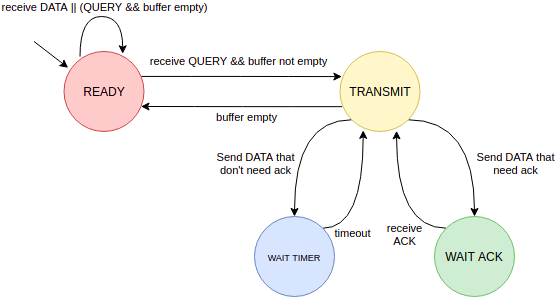
\includegraphics[scale=0.5]{res/pictures/loramac-loraroot-state.drawio.png}
        \caption{Diagramme d'état de la racine LoRa.}
        \label{fig:archi-state-lora}
    \end{figure}

\subsection*{Construction du réseau}%done
    A l'initialisation du réseau, une racine RPL doit envoyer une trame avec la commande JOIN. Une 
    fois reçue par la racine LoRa, celle-ci va répondre avec une trame JOIN\_RESPONSE qui fait 
    office d'acquittement de la trame JOIN et dont la payload est le préfixe du réseau de la racine 
    RPL qu'elle doit diffuser dans son réseau.

    Si la trame JOIN ou la trame JOIN\_RESPONSE ne sont pas reçues, la racine RPL retransmettra la 
    trame JOIN à l'expiration d'un timer \textit{retransmit\_timer} déclenché à l'envoi de la trame 
    JOIN. Cette retransmission se répète au maximum \textsc{max\_attempt} fois. Si ce seuil est 
    dépassé, la communication est considirée comme échouée. Dans ce cas, la racine attend $w$ 
    secondes avant de répéter le processus. $w$ est défini par l'équation~\ref{eq:archi-wait}, 
    dans laquelle, $r$ est le temps ajouté au $retransmit\_timeout$ qui est le temps après lequel 
    le timer \textit{retransmit\_timer} expire. $r$ est le modulo $retransmit\_timeout$ d'un nombre 
    $rand$ qui doit être choisi aléatoirement.
    \begin{equation}\label{eq:archi-wait}
        \begin{split}
            r = rand \% retransmit\_timeout \\
            w = (retransmit\_timeout + r) \% 60
        \end{split}
    \end{equation}
    
    Une fois le préfixe reçu, la racine RPL peut initialiser le réseau RPL et y diffuser le préfixe.

    Le diagramme de séquence de la figure~\ref{fig:proto-seq-join} illustre le processus de construction du réseau.
    \begin{figure}[H]
        \centering
        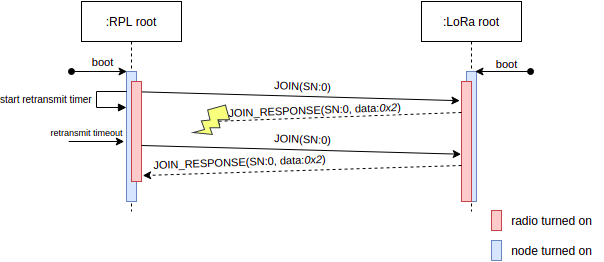
\includegraphics[scale=0.6]{res/pictures/loramac-sequence-JOIN.drawio.png}
        \caption{Diagramme de séquence de la construction du réseau.}
        \label{fig:proto-seq-join}
    \end{figure}

\subsection*{Communications montantes}%done
    Lorsq'un paquet est destiné à une adresse IPv6 externe au réseau d'une racine RPL, il va remonter jusqu'à celle-ci, qui va ensuite l'envoyer à la racine LoRa.

    Si la trame envoyée à la racine LoRa nécessite un acquittement, la racine RPL n'enverra pas d'autres trames tant que l'acquittement n'a pas été reçu (état \textit{wait\_response}).
    A l'envoi de cette trame, le timer \textit{retransmit\_timer} est déclenché. S'il expire avant que l'acquittement ne soit reçu, la trame sera retransmise pour un maximum de 3 fois.
    Arpès 3 transmissions qui n'ont pas réussi, la racine RPL retourne dans l'état READY et le paquet est perdu.

    Si la trame envoyée à la racine LoRa ne nécessite pas d'acquittement, la réception ne cette trame n'est pas garantie et la racine RPL peut directement transmettre les trames suivantes s'il y en a.

    Le diagramme de séquence de la figure~\ref{fig:proto-seq-upward} illustre le déroulement des communications montantes.
    \begin{figure}[H]
        \centering
        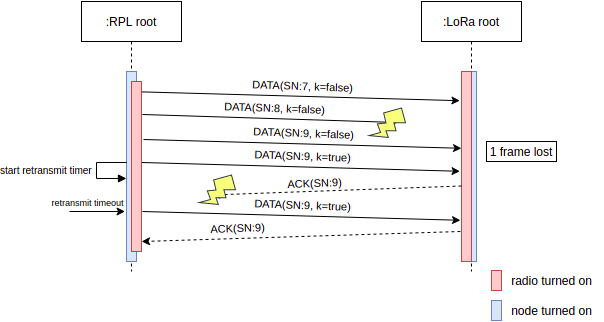
\includegraphics[scale=0.6]{res/pictures/loramac-sequence-UPWARD.drawio.png}
        \caption{Diagramme de séquence du trafique montant.}
        \label{fig:proto-seq-upward}
    \end{figure}    

\subsection*{Communications Descendantes}%done
    La racine LoRa possède un buffer pour chaque réseau RPL dans lequel elle accumule les paquets destinés à ce réseau. Pour chaque racine RPL, lors de l'expiration, à intervalle régulier, du timer \textit{query\_timer}, une trame avec la commande QUERY est transmise à la racine LoRa.

    La réponse à cette trame doit être un acquittement, si la racine LoRa n'a pas de paquets pour le réseau de cette racine RPL, ou une trame avec la commande DATA si un ou plusieurs paquets sont disponibles.

    Si la racine LoRa possède plusieurs paquets à destination du même réseau RPL, la valeur du flag \textit{next} doit être à 1 pour toutes les trames envoyées à l'exception de la dernière.

    Comme pour les communications montantes, les retransmissions sont initiées par les racines RPL.
    Le timer \textit{retransmit\_timer} est activé lorsque la QUERY est envoyée ou lorsqu'une trame DATA avec le flag \textit{next} à 1 est reçue.

    Les acquittements ne sont pas nécessaire pour les communications descendantes, car quand la racine LoRa envoi une trame, cela signifie qu'une racine RPL attend cette trame. Si elle n'est pas reçue, la racine RPL demandera une retransmission via l'envoi de la dernière trame envoyée, c'est à dire la trame avec la commande QUERY.

    Après 3 retransmissions, le paquet est perdu et le prochain sera transmis lors de la réception d'une QUERY.

    Le diagramme de séquence de la figure~\ref{fig:proto-seq-downward} illustre le déroulement des communications descendantes.
    \begin{figure}[H]
        \centering
        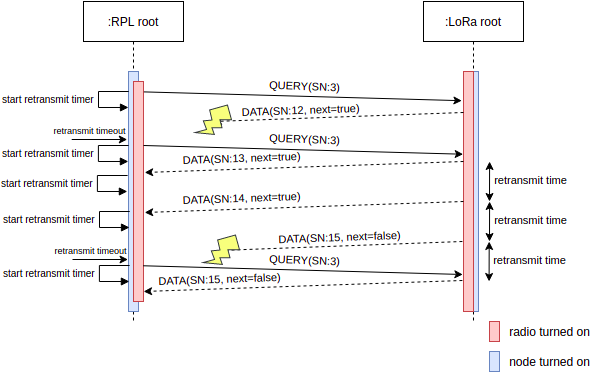
\includegraphics[scale=0.6]{res/pictures/loramac-sequence-DOWNWARD.drawio.png}
        \caption{Diagramme de séquence du trafique descendant.}
        \label{fig:proto-seq-downward}
    \end{figure}


    %Si une trame nécessite un acquittement et que l'acquittement n'est pas reçu, la racine LoRa %n'envoie pas le paquet suivant. Dans ce cas deux situations sont possibles:
    %\begin{itemize}
    %    \item La trame avait le flag \textit{next} à 1:\\
    %        La racine RPL s'attend à une autre trame. L'acquittement va donc être retransmis à %l'expiration du \textit{retransmit\_timer} avec un maximum 3 retransmissions.
    %    \item La trame avait le flag \textit{next} à 0:\\
    %        La racine LoRa retransmettra le paquet concerné lors de la réception d'une QUERY.
    %\end{itemize}

\subsection*{Gestion des numéros de séquence}
    Les racines RPL et la racine LoRa possèdent deux compteurs: \textit{expected\_sn} et \textit{next\_sn}.

    La valeur du compteur \textit{expected\_sn} est le numéro de séquence attendu de la prochaine trame reçue. Ce compteur permet de savoir si une trame a été perdue. Sa valeur est le numéro de séquence de la dernière trame reçue incrémenté de 1.

    La valeur du compteur \textit{next\_sn} est le numéro de séquence de la prochaine trame. Il est incrémenté de 1 lorsqu'une trame a été envoyée.

    Les deux compteurs sont initialisés à zéro.

%\subsubsection*{Exemple de communications}
%    Les figures~\ref{fig:archi-sequence1} et~\ref{fig:archi-sequence2} ci-dessous, illustrent le 
%    protocole LoRaMAC qui vient d'être décrit dans cette section. La première illustre les échanges 
%    de messages sans retransmissions et la deuxième avec retransmissions. Les détails des timers ne 
%    sont pas présents sur ces figures pour plus de clarté.
%    \begin{figure}[H]
%        \centering
%        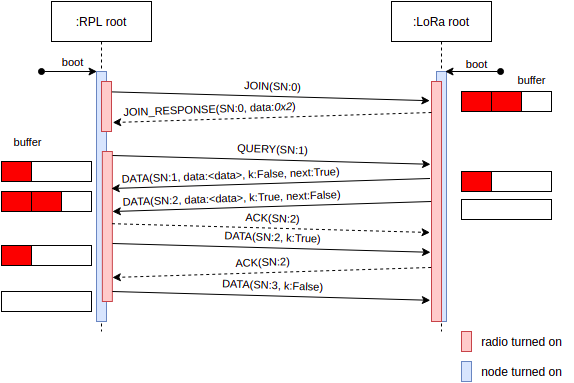
\includegraphics[scale=0.6]{res/pictures/loramac-sequence1.drawio.png}
%        \caption{Diagramme de séquence LoRaMAC.}
%        \label{fig:archi-sequence1}
%    \end{figure}
%    \begin{figure}[H]
%        \centering
%        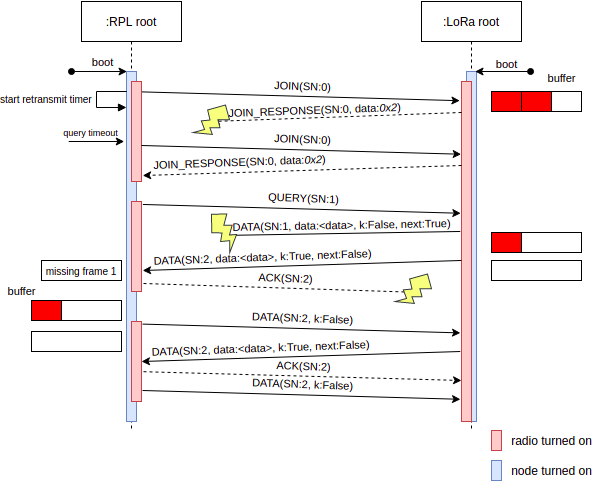
\includegraphics[scale=0.6]{res/pictures/loramac-sequence2.drawio.png}
%        \caption{Diagramme de séquence LoRaMAC avec retransmissions.}
%        \label{fig:archi-sequence2}
%    \end{figure}

%\subsection{Evitement de collision}
%    L'envoi des trames est réalisé avec l'algorithme CSMA/CA pour les racines RPL. 
%    Avant l'envoi, ces noeuds écoute le canal. Si le canal est occupé, le noeud va resonder le
%    canal après un temps aléatoire. Ce processus se répète 3 fois. Après ces trois fois, si le
%    canal est toujours occupé, la trame ne sera pas envoyée. A chaque sondage du canal, l'interval
%    dans lequel le temps aléatoire est choisi est agrandit. Si le canal n'est pas occupé, la trame
%    est envoyée.
